\chapter{Risultati e Conclusioni}
\begin{figure}[h]
	\centering
		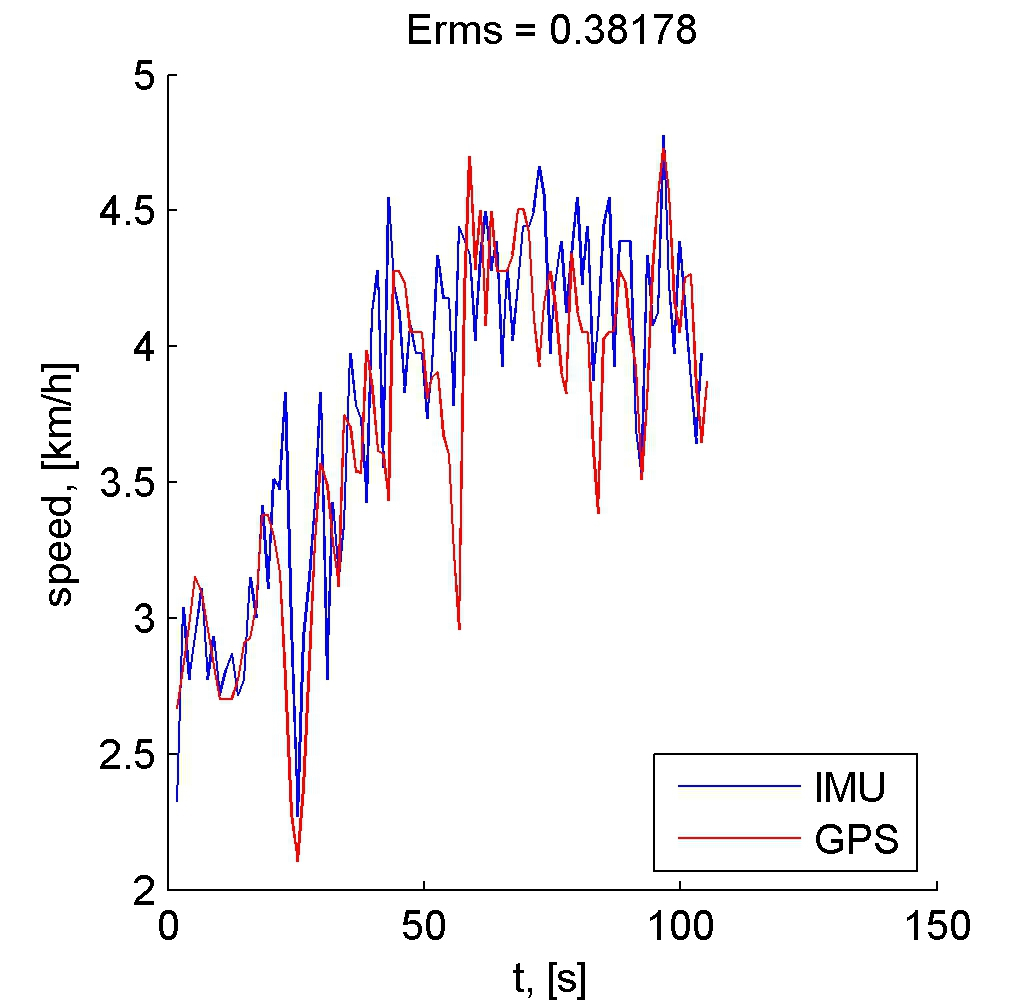
\includegraphics[width=.8\textwidth]{imgs/speedSVR4.jpg}
	\caption{Confronto fra le due velocit� $IMUspeed$ (traccia rossa) e $GPSspeed$ (traccia blu) rispetto al tempo in $Km/h$ in funzione del tempo in secondi. Mostra una forte somiglianza tra tra le due velocit�.}
	\label{fig:IMUspeedGPSspeedVStime}
\end{figure}
\begin{figure}
	\centering
		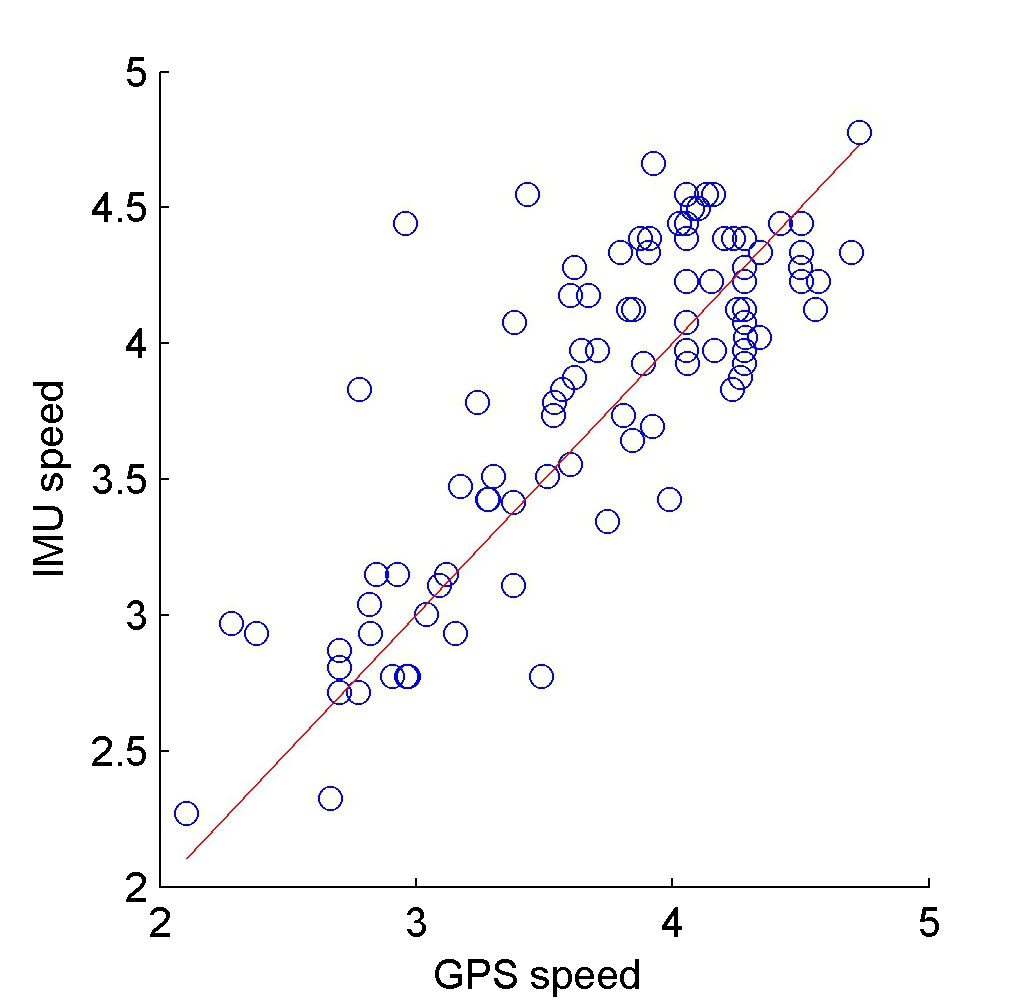
\includegraphics[width=.8\textwidth]{imgs/speedSVR5.jpg}
	\caption{Grafico a dispersione (\textit{scatter plot}) delle due velocit� $IMUspeed$ e $GPSspeed$. Mostra come ci sia una buona corrispondenza fra i due gruppi di valori.}
	\label{fig:IMUspeedVSGPSspeed}
\end{figure}

\begin{figure}
	\centering
		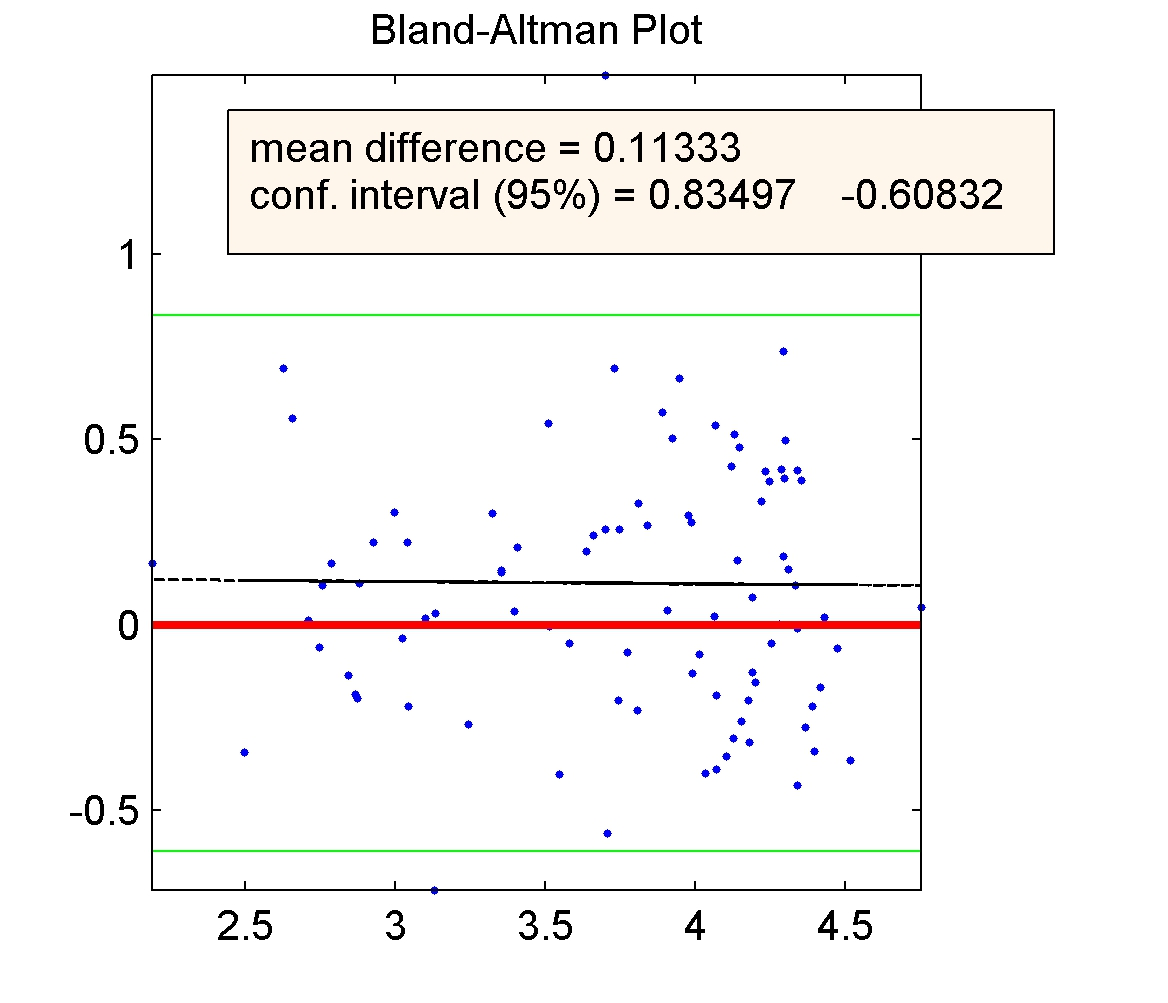
\includegraphics[width=.8\textwidth]{imgs/speedSVRBlandAltmann.jpg}
	\caption{Confronto fra le due velocit� $IMUspeed$ e $GPSspeed$ mediante un Bland Altman \textit{plot} o grafico a differenza o grafico delle differenze medie. La linea rossa rappresenta la linea a differenza nulla, la linea nera la differenza media, mentre le linee verdi la deviazione standard (o intervallo di confidenza). Il 95\% dei valori sta all'interno dell'intervallo di confidenza. }
	\label{fig:IMUspeedVSGPSspeedBA}
\end{figure}

\begin{figure}
	\centering
		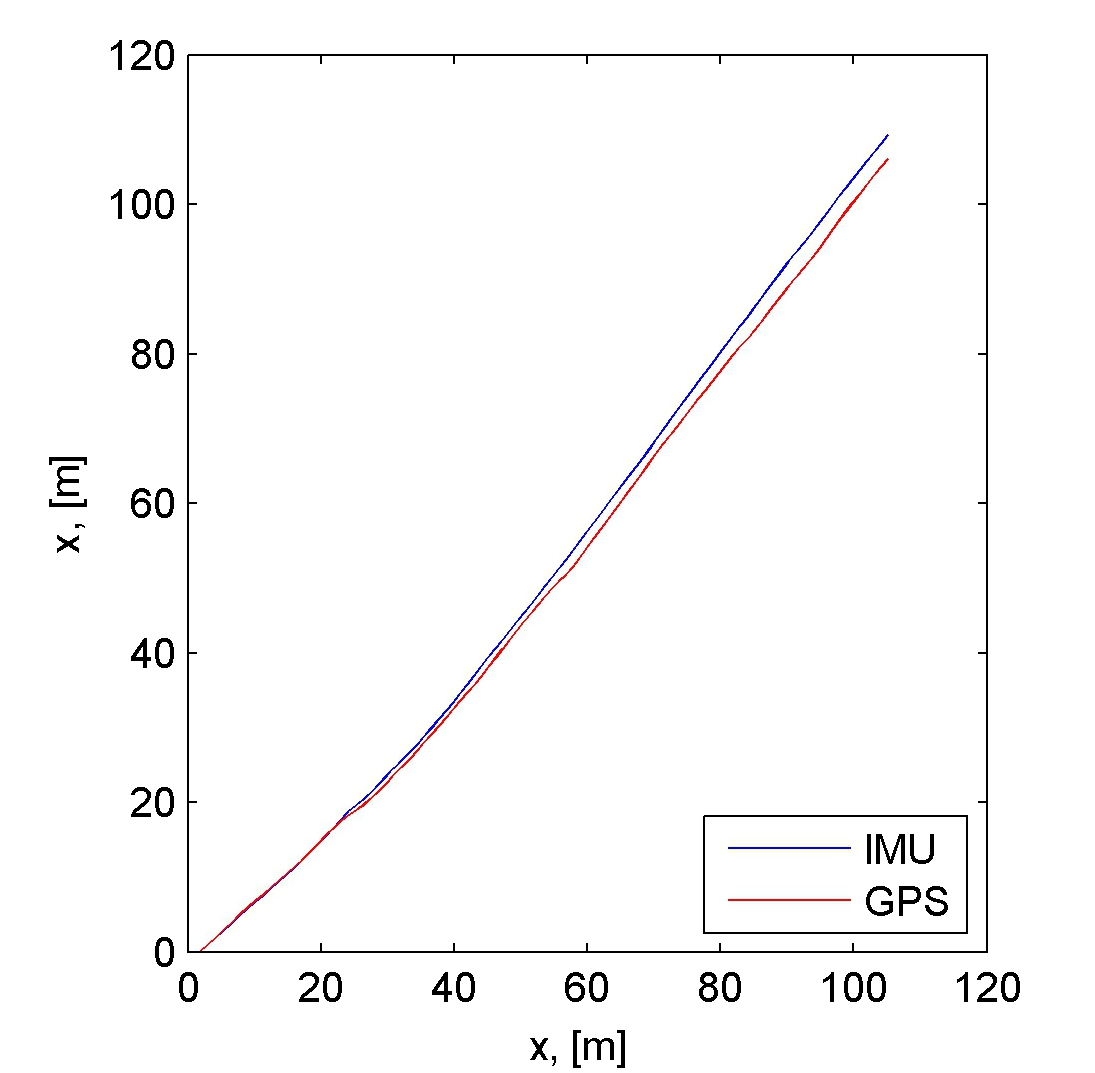
\includegraphics[width=.8\textwidth]{imgs/displSVR1.jpg}
	\caption{Confronto fra le due distanze $IMUdistance$ (traccia blu) e $GPSdistance$ (traccia rossa) rispetto al tempo. Mostra che la IMU sovrastima la distanza. Al termine dell'esperimento (a circa $110m$ di distanza percorsa) l'errore � commesso � di circa $5m$.}
	\label{fig:IMUdistanceGPSdistanceVStime}
\end{figure}

\begin{figure}
	\centering
		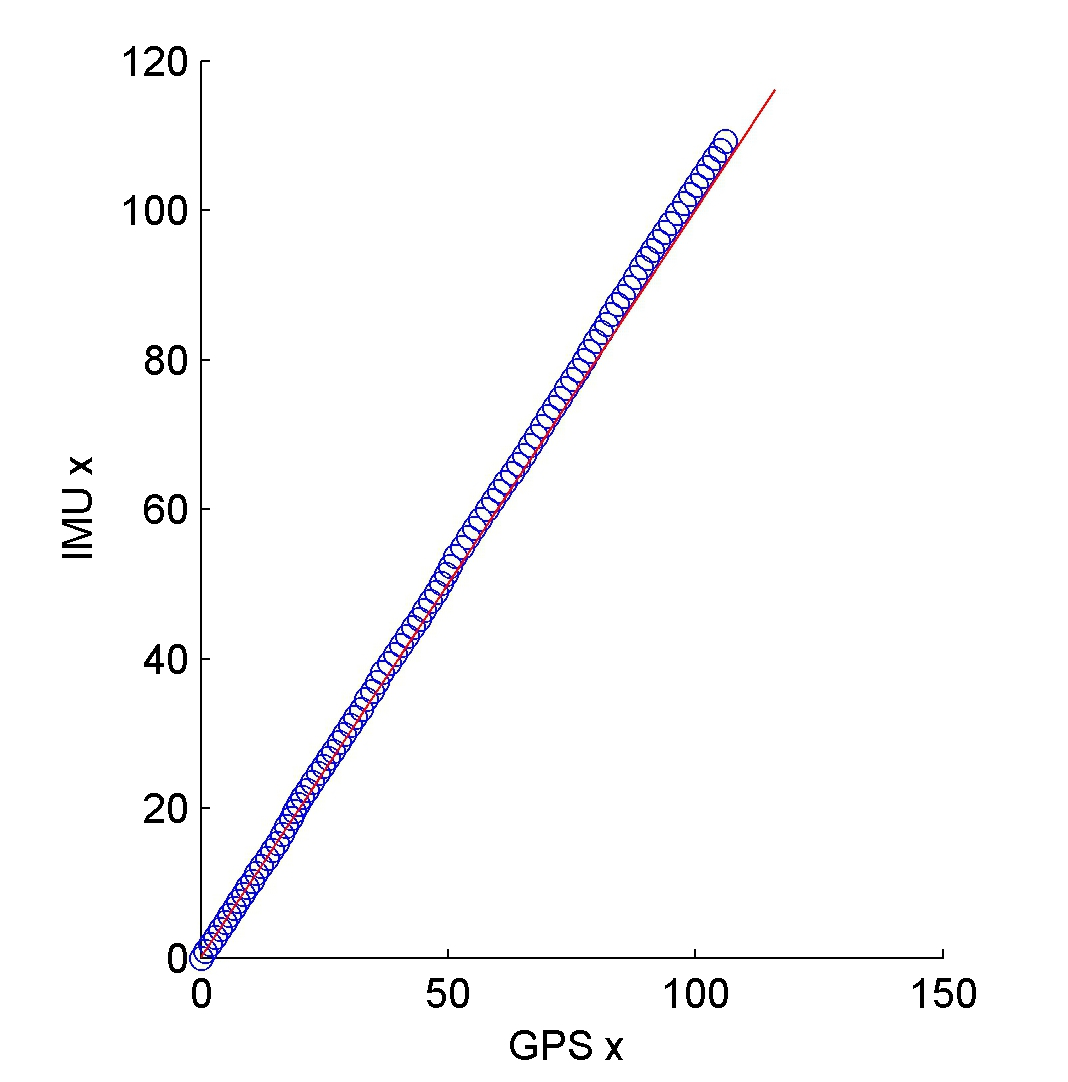
\includegraphics[width=.8\textwidth]{imgs/displSVR2.jpg}
	\caption{Grafico a dispersione delle due distanze $IMUdistance$ e $GPSdistance$ mostra una elevato grado di allineamento fra le distanze misurate con i due strumenti.}
	\label{fig:IMUdistanceVSGPSdistance}
\end{figure}

